\documentclass{beamer}

\usepackage{color}
\definecolor{ForestGreen}{RGB}{60, 128, 49}
\definecolor{Blue}{RGB}{45, 47, 146}

\usetheme[menuwidth={0.3\paperwidth}]{erlangen}
\setbeamercovered{transparent=20}

\begin{document}

\title[Interpretation of natural language instructions]{Interpretation of natural language instructions} 
\subtitle{Translating sentences by using a grammar}
\author{Martin Agfjord} 
\date{\today} 
\institute{University of Gothenburg\\ 
  \vspace{-0.2em}{\small Computer Science  and Engineering} }

\begin{frame}[plain]
    \thispagestyle{empty}

  \begin{picture}(0,0)(0,0)
    \put(-29,-171){
\includegraphics[width=1.01\paperwidth]{images/titlepage2.pdf}}
  \end{picture}

  \begin{picture}(0,0)(0,0)
    \put(10,0){
        \begin{minipage}{0.9\linewidth}
        \centering{\LARGE\color{erlangenwhite} \inserttitle\par}
        \vspace{5mm}
        \centering{\large\color{erlangenlightgrey} \insertsubtitle\par}
        \end{minipage}
    }
  \end{picture}
  \begin{picture}(0,0)(0,0)
    \put(10,-65){
        \begin{minipage}{0.90\linewidth}
        \centering{\large\color{erlangenwhite} \insertauthor\par}
        \end{minipage}
    }
  \end{picture}
  \begin{picture}(0,0)(0,0)
    \put(10,-127){
        \begin{minipage}{0.90\linewidth}
        \centering{\color{erlangenblue} \insertinstitute\par}
        \end{minipage}
    }
  \end{picture}
\end{frame}

\begin{frame}{Outline}
  \tableofcontents
\end{frame}

\section{Introduction \& problem description}
\begin{frame}{Introduction \& problem description} 
    \begin{itemize}
    \item An alternative user interface \pause
    \item Translation \pause % from natural language to query language
    \item Delimitation 
      \begin{itemize}
        \item Intranet of a software development company \pause
        \item Customers, People and Projects exists \pause
	    \item Limited amount of instructions
      \end{itemize}
  \end{itemize} 
\end{frame}

\begin{frame}{Interface definition} 
\begin{block}{Sufficient for novice users}
      \texttt{people who know Java}
\end{block}
\pause
\begin{block}{Sufficient for expert users}
      \texttt{people java}
\end{block}
\end{frame}

\section{Solution} 
\begin{frame}{Solution} 
  \begin{itemize}
    \item Precise translation \pause
    \item Need mapping from natural language to query language \pause
      \begin{itemize}
        \item Use a grammar
      \end{itemize}
  \end{itemize}
  
\end{frame}

\begin{frame}{Translation with a grammar} 
         \begin{itemize}
		   \item Structured rules for strings \pause
           \item Example: Is/Are rule \pause
           \begin{itemize}
             \item The students \textcolor{String}{are} here
             \item The student \textcolor{String}{is} here \pause
           \end{itemize}             
           \item Swedish
           \begin{itemize}
             \item Studenterna \textcolor{String}{{\"a}r} h{\"a}r
             \item Studenten \textcolor{String}{{\"a}r} h{\"a}r \pause
           \end{itemize}\pause
           \item Use the rules to capture the meaning of a sentence\pause
           \begin{itemize}
             \item Studenterna {\"a}r h{\"a}r \texttt{===> (Def Student\_Plural\ Is Here)}\pause
           \end{itemize}
           \item Use the rules again to produce a sentence \pause
           \begin{itemize}
             \item \texttt{(Def Student\_Plural Is Here) ===>} The students are here \pause
           \end{itemize}
         \end{itemize}
           \begin{block}{How can we build a grammar to translate sentences?}
              We will use Grammatical Framework (GF)
         \end{block}
\end{frame}
%###################################
%                     GF INTRODUCTION
%###################################
\begin{frame}{Introducing Grammatical Framework (GF)} 
         \begin{itemize}
           \item Open source development platform for natural languages \pause
           \begin{itemize}
              \item Functional programming language \pause
              \item Designed for creating natural language grammars
               %specifically designed for writing grammars.
           \end{itemize}\pause
           \item Separates abstract and concrete syntax \pause
           \begin{itemize}
              \item Abstract syntax captures the \emph{logic} of a sentence \pause
              % It is a tree!
              \item Concrete syntax represents the logic as a string
           \end{itemize}\pause
         \end{itemize}
         
           \begin{block}{Same technique used by programming languages}
             \begin{itemize}
               \item Programmer writes source code in concrete syntax \pause
               \item Compiler translates concrete syntax to abstract syntax \pause
               \item The rest of the compiler manipulates the abstract syntax
             \end{itemize}
         \end{block}
         
\end{frame}

\begin{frame}[fragile]{A simple example}
\textbf{Abstract syntax}
\begin{semiverbatim}
Instruction People (Know Java)

    Instruction
   /           \\
People        Know
                |
              Java
\end{semiverbatim}\pause


\textbf{Concrete syntaxes}
\begin{semiverbatim}
people who know Java                           -- English
personer som kan Java                          -- Swedish
q=object_type : Person AND expertise : Java    -- Solr
\end{semiverbatim}
\end{frame}

\begin{frame}[fragile]{GF implementation: Abstract syntax}\pause
\begin{semiverbatim}
abstract Instrucs = \{
  cat \textcolor{ForestGreen}{
    Instruction 
    Subject ;
    Relation ;
    Object ; }\pause
  fun \textcolor{Blue}{
    MkInstruction : Subject -> Relation -> Instruction ;
    People : Subject ;
    Know : Object -> Relation ;
    Java : Object }
\}
\end{semiverbatim}
\end{frame}

\begin{frame}[fragile]{GF implementation: English concrete syntax}\pause
\begin{semiverbatim}
concrete InstrucsEng of Instrucs = \{
  lincat \textcolor{ForestGreen}{
    Instruction = \textcolor{Type}{Str} ;
    Subject = \textcolor{Type}{Str} ;
    Relation = \textcolor{Type}{Str} ;
    Object = \textcolor{Type}{Str} ; }\pause
  lin \textcolor{Blue}{
    MkInstruction subject relation = 
                   subject ++ \textcolor{String}{"who"} ++ relation ;
    People = \textcolor{String}{"people"} ;
    Know object = \textcolor{String}{"know"} ++ object ;
    Java = \textcolor{String}{"Java"} ; }
\}
\end{semiverbatim}
\end{frame}

\begin{frame}[fragile]{GF implementation: Solr concrete syntax}\pause
\begin{semiverbatim}
concrete InstrucsEng of Instrucs = \{
  lincat \textcolor{ForestGreen}{
    Instruction = \textcolor{Type}{Str} ;
    Subject = \textcolor{Type}{Str} ;
    Relation = \textcolor{Type}{Str} ;
    Object = \textcolor{Type}{Str} ;}\pause
  lin \textcolor{Blue}{
    MkInstruction subject relation = 
                   \textcolor{String}{"q="} ++ subject ++ \textcolor{String}{"AND"} ++ relation ;
    People = \textcolor{String}{"object_type : Person"} ;
    Know object = \textcolor{String}{"expertise : "} ++ object ;
    Java = \textcolor{String}{"Java"} ; }
\}
\end{semiverbatim}
\end{frame}

\begin{frame}[fragile]{GF implementation: Translation}
GF + Abstract syntax + Concrete syntax = \pause
\newline
\newline
\textbf{Parser}
\begin{semiverbatim}
> parse -lang=InstrucsEng \textcolor{String}{"people who know Java"}
MkInstruction People (Know Java)
\end{semiverbatim} \pause
\textbf{Linearizer}
\begin{semiverbatim}
> linearize -lang=InstrucsSolr 
>                  MkInstruction People (Know Java)
\textcolor{String}{"q= object_type : Person AND expertise : Java"}
\end{semiverbatim} \pause
\textbf{Generator}
\begin{semiverbatim}
> generate_trees
MkInstruction People (Know Java)
\end{semiverbatim}
\end{frame}
%###################################
%                  GF RESOURCE GRAMMAR LIBRARY
%###################################
\begin{frame}[fragile]{GF implementation: Resource Grammar Library}\pause
\begin{itemize}
\item Contains linguistic descriptions for natural languages\pause
  \begin{itemize}
    \item Types for nouns, verbs, adjectives, noun phrases, verb phrases, relative sentences, phrases...\pause
  \end{itemize}
  \item Developer does not need to know linguistics\pause
  \begin{itemize}
      \item Example: 'Yesterday I ate an apple' \pause
      \item Direct translation to Swedish: 'Ig{\aa}r \textcolor{ForestGreen}{jag} \textcolor{String}{{\aa}t} ett {\"a}pple' \pause
      \item Correct translation to Swedish: 'Ig{\aa}r \textcolor{String}{{\aa}t} \textcolor{ForestGreen}{jag} ett {\"a}pple' \pause
      \end{itemize}
  \item Only need to know the \emph{domain}
\end{itemize}
\end{frame}
\begin{frame}[fragile]{Resource Grammar Library: English concrete syntax} \pause
\begin{semiverbatim}
concrete InstrucsEng of Instrucs = {
  lincat\textcolor{ForestGreen}{
    Instruction = \textcolor{Type}{NP} ;
    Subject = \textcolor{Type}{N} ;
    Relation = \textcolor{Type}{RS} ;
    Object = \textcolor{Type}{NP} ;}\pause

  lin \textcolor{Blue}{
   MkInstruction subject relation = 
                    mkNP aPl_Det (mkCN subject relation) ;
   People = mkN \textcolor{String}{"person" "people"} ;
   Know object = mkRS' (mkVP (mkV2 (mkV \textcolor{String}{"know"})) object) ;
   Java = mkNP (mkPN \textcolor{String}{"Java"}) ; }
  oper
     mkRS' : \textcolor{Type}{VP} -> \textcolor{Type}{RS} = \\vp -> mkRS (mkRCl which_RP vp) ;
}
\end{semiverbatim}
\end{frame}

\begin{frame}[fragile]{Resource Grammar Library: Swedish concrete syntax}
\begin{semiverbatim}
concrete InstrucsEng of Instrucs = {
  lincat\textcolor{ForestGreen}{
    Instruction = \textcolor{Type}{NP} ;
    Subject = \textcolor{Type}{N} ;
    Relation = \textcolor{Type}{RS} ;
    Object = \textcolor{Type}{NP} ;}

  lin\textcolor{Blue}{
   MkInstruction subject relation = 
                    mkNP aPl_Det (mkCN subject relation) ;
   People = mkN \textcolor{String}{"person" "personer"} ;
   Know object = mkRS' (mkVP (mkV2 (mkV \textcolor{String}{"kan"}) object)) ;
   Java = mkNP (mkPN \textcolor{String}{"Java"}) ; }
  oper
     mkRS' : \textcolor{Type}{VP} -> \textcolor{Type}{RS} = \\vp -> mkRS (mkRCl which_RP vp) ;
}
\end{semiverbatim}
\end{frame}

\begin{frame}{}
    \sectionframe{Extending the grammar}
\end{frame}

%###################################
%                  EXTENDING THE GRAMMAR:
%                  NAMES
%###################################
\begin{frame}[fragile]{Extending the grammar: All programming languages}
\begin{itemize}
\item Extend the grammar to support more programming languages\pause
\item Arbitrary names instead of hard coded functions
\end{itemize}
\begin{semiverbatim}
fun
  \textcolor{Blue}{Java : Object ; }
lin
  \textcolor{Blue}{Java = \textcolor{String}{"Java"} ; }
\end{semiverbatim}\pause

\texttt{===>}

\begin{semiverbatim}
fun
  \textcolor{Blue}{MkObject : Symb -> Object ; }
lin
  \textcolor{Blue}{MkObject symb = symb.s ; }
\end{semiverbatim}
\end{frame}
%###################################
%                  EXTENDING THE GRAMMAR:
%                  MORE INSTRUCTIONS
%###################################
\begin{frame}[fragile]{Extending the grammar: More instructions}
\begin{itemize}
\item Extend grammar to support more instructions\pause
\item Support \textbf{valid} sentences regarding \emph{customers}, \emph{people} and \emph{projects}:\pause
\end{itemize}
  \vspace{-4mm}\begin{itemize}
    \item[] \texttt{people who know Java}
    \item[] \texttt{people who work in London}
    \item[] \texttt{people who work with Unicef}
    \item[] \texttt{customers who use Solr}
    \item[] \texttt{projects who use Solr}
  \end{itemize}\pause
  \begin{itemize}
    \item Not support invalid sentences, for instance:
  \end{itemize}
   \vspace{-4mm}\begin{itemize}
    \item[] \texttt{projects who work in London}
    \item[] \texttt{people who use Solr}
    \item[] \texttt{customers who work with Unicef}
  \end{itemize}
\end{frame}

\begin{frame}[fragile]{Extending the grammar: More instructions}
\begin{itemize}
\item Resolved by adding more categories (types)
\end{itemize}

\vspace{-4mm}\begin{semiverbatim}\small
cat \textcolor{ForestGreen}{
  Internal ; External ; Resource ;
  InternalRelation ; ExternalRelation ; ResourceRelation ; }\pause
fun \textcolor{Blue}{
  People   : Internal ;
  Customer : External ;
  Project  : Resource ; }\pause
  \textcolor{Type}{
  Know     : Object -> InternalRelation ;
  UseExt   : Object -> ExternalRelation ;
  UseRes   : Object -> ResourceRelation ;}\pause
  \textcolor{String}{
  InstrucInternal : Internal -> InternalRelation -> Instruction ;
  InstrucExternal : External -> ExternalRelation -> Instruction ;
  InstrucResource : Resource -> ResourceRelation -> Instruction ; }
\end{semiverbatim}
\end{frame}
%###################################
%                  EXTENDING THE GRAMMAR:
%                  BOOLEAN OPERATORS
%###################################
\begin{frame}[fragile]{Extending the grammar: Boolean operators}\pause
\begin{itemize}
  \item Extend grammar to support boolean operators
  \item \texttt{people who know Java and Python} \pause
  \item \texttt{people who know Java or work in London} \pause
\end{itemize}
\begin{semiverbatim}
fun \textcolor{Blue}{
  And : Object -> Object -> Object ;
  Or : Object -> Object -> Object ;}
\end{semiverbatim}

\begin{semiverbatim}
lin\textcolor{Blue}{
  And o1 o2 = o1 ++ \textcolor{String}{"and"} ++ o2 ;
  Or o1 o2 = o1 ++ \textcolor{String}{"or"} ++ o2 ;}
\end{semiverbatim}
\end{frame}
%###################################
%                  SUGGESTION ENGINE:
%                  
%###################################
\begin{frame}[fragile]{Suggestion Engine}
\begin{itemize}
\item Narrow application grammar requires precise input\pause
\item Need to help user to find correct instructions\pause
\item Use suggestions based on partial input\pause
\item Extract possible instructions into Solr\pause
\end{itemize}
\textbf{Problem with arbitrary names}
\begin{semiverbatim}\small
\only<1-5>{






} \pause \only<6>{
> generate_trees
InstrucExternal Customer (UseExt (MkObject (MkSymb \textcolor{String}{"Foo"})))
InstrucInternal People (Know (MkObject (MkSymb \textcolor{String}{"Foo"})))
InstrucInternal People (WorkIn (MkObject (MkSymb \textcolor{String}{"Foo"})))
InstrucInternal People (WorkWith (MkObject (MkSymb \textcolor{String}{"Foo"})))
InstrucResource Project (UseRes (MkObject (MkSymb \textcolor{String}{"Foo"})))
} \pause \only<7>{
> generate_trees | linearize -lang=InstrucsEng
\textcolor{String}{"customers who use \textcolor{Type}{Foo}"
"people who know \textcolor{Type}{Foo}"
"people who work in \textcolor{Type}{Foo}"
"people who work with \textcolor{Type}{Foo}"
"projects which use \textcolor{Type}{Foo}"}
}
\end{semiverbatim}

\end{frame}

\begin{frame}[fragile]{Suggestion Engine}
\begin{itemize}
\item Resolved by introducing name types
\end{itemize}
\begin{semiverbatim}
MkSkill : Symb -> Skill ;
MkOrganization : Symb -> Organization ;
MkModule: Symb -> Module ;
MkLocation : Symb -> Location
\end{semiverbatim}
\begin{semiverbatim}\footnotesize
\only<1>{






}\only<2>{
> generate_trees
InstrucExternal Customer (UseExt (\textcolor{Type}{MkModule} (MkSymb \textcolor{String}{"Foo"})))
InstrucInternal People (Know (\textcolor{Type}{MkSkill} (MkSymb \textcolor{String}{"Foo"})))
InstrucInternal People (WorkIn (\textcolor{Type}{MkLocation} (MkSymb \textcolor{String}{"Foo"})))
InstrucInternal People (WorkWith (\textcolor{Type}{MkOrganization} (MkSymb \textcolor{String}{"Foo"})))
InstrucResource Project (UseRes (\textcolor{Type}{MkModule} (MkSymb \textcolor{String}{"Foo"})))
}\pause \only<3>{
> generate_trees (post processed)
InstrucExternal Customer (UseExt (\textcolor{Type}{MkModule} (MkSymb \textcolor{String}{"Module0"})))
InstrucInternal People (Know (\textcolor{Type}{MkSkill} (MkSymb \textcolor{String}{"Skill0"})))
InstrucInternal People (WorkIn (\textcolor{Type}{MkLocation} (MkSymb \textcolor{String}{"Location0"})))
InstrucInternal People (WorkWith (\textcolor{Type}{MkOrganization} (MkSymb \textcolor{String}{"Organi..})))
InstrucResource Project (UseRes (\textcolor{Type}{MkModule} (MkSymb \textcolor{String}{"Module0"})))
} \pause \only<4>{
> generate_trees | linearize -lang=InstrucsEng
\textcolor{String}{"customers who use \textcolor{Type}{Module0}"
"people who know \textcolor{Type}{Skill0}"
"people who work in \textcolor{Type}{Location0}"
"people who work with \textcolor{Type}{Organization0}"
"projects which use \textcolor{Type}{Module0}"}
}
\end{semiverbatim}

\end{frame}

\begin{frame}[fragile]{Suggestion Engine: Pseudocode of algorithm}\pause
\begin{semiverbatim}\small
suggestions(sentence) \{
    \textcolor{Comment}{// sentence = "anyone that ever knew java"
    // names[] = \{Java\}}
    names[] = extractNames(sentence);\pause
    \vspace{-2mm} \textcolor{Comment}{
    // "anyone that ever knew java" ===> 
    // "anyone that ever knew Skill0"}
    sentence = replaceNamesWithTypes(sentence, names); \pause
    \vspace{-2mm}\textcolor{Comment}{
    // suggestions = \{ "people who know Skill0", ... \} }
    suggestions[] = findSentences(sentence);\pause
    \vspace{-2mm}
    for each suggestion in suggestions \{ \textcolor{Comment}{
    // "people who know Skill0" ===> 
    // "people who know Java"}
      suggestion = restoreNames(names, suggestion);
    \}
    return suggestions; 
\}
\end{semiverbatim}
\end{frame}

\section{Results} 
\begin{frame}{Results}
\begin{center}
\only<1>{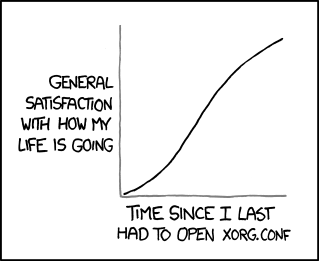
\includegraphics[scale=0.6,keepaspectratio,valign=t]{./images/x11.png}}\pause
\only<2>{
\includegraphics[scale=0.6,keepaspectratio,valign=t]{./images/graph.png}}
\end{center}
\end{frame}

\section{Conclusion} 
\begin{frame}{Conclusion}\pause
\begin{itemize}
\item Application sufficient for novice and expert users \pause
\item Resource Grammar Library not worth the effort\pause
  \begin{itemize}
    \item Not possible to express a few sentences\pause
    % For example
    % people that know java
    % people who know java and work in Gothenburg
    \item Problem with constant \texttt{which\_RP}\pause
    \item Linearizes \texttt{projects \textcolor{String}{who} use Solr}\pause  
  \end{itemize}
\end{itemize}
\end{frame}

\begin{frame}{Future Work}\pause
\begin{itemize}
\item Improvments of suggestions \pause
\item Instructions in speech \pause
\item Proper handling of ambiguous instructions
\item Use application in other context
\end{itemize}
\end{frame}

\end{document}
